\section{Study 1: Field Study on the Effect of Rotating Interventions}

Our first study is a within-subjects design run on the HabitLab platform that aims to understand the effects of rotating interventions on effectiveness and attrition.

\subsection{Participants}

% todo confirm it was actually 3 weeks

% Participants in our first study consisted of new HabitLab users installing the system over a period of three weeks in March and April 2018. 217 users installed HabitLab over the course of our experiment and consented to our research protocol. We discarded participants who were not new users of HabitLab, since some users were reinstalls or new devices for existing users. We also discarded participants who did not the complete the onboarding process, or who uninstalled the system before they saw their first intervention.

Participants in our first study consisted of new HabitLab users installing the system over a period of three weeks in March and April 2018. 692 users installed HabitLab over the course of our experiment and consented to our research protocol. We discarded participants who were not new users of HabitLab, since some users were reinstalls or new devices for existing users. We also discarded participants who did not the complete the onboarding process, or who uninstalled the system before they saw their first intervention. This left us with 217 participants. %\msb{didn't we also filter out people who manipulated the default settings?} \gezacomment{no that was the other study, this one bypassed that issue because the static selection algorithm continued choosing the same intervention even if they had multiple enabled} % For this study, we focus only on users who enabled interventions for Facebook. This final subset consists of 55 participants.

% Participants in our first study consisted of new HabitLab users installing the system over a period of three weeks in March and April 2018. 217 users installed HabitLab over the course of our experiment and consented to our research protocol. We discarded participants who were not new users of HabitLab, since some users were reinstalls or new devices for existing users. We also discarded participants who did not the complete the onboarding process, or who uninstalled the system before they saw their first intervention. For this study, we focus only on users who enabled interventions for Facebook. This final subset consists of 55 participants. \msb{didn't we also filter out people who manipulated the default settings?} \gezacomment{no that's study 0 which we're leaving out of this paper} % \msb{they are users in the context of a system; participants in the context of a study} 

% are reviewers not going to like that our userbase is 89% male?

%\msb{general rule: do not use parentheticals in writing. either 1) the statement is important enough to be a full member of the sentence, in which case you should promote it out of the parens; or 2) it's not important enough to be a full member, in which case you should cut it. I'm editing out a ton of parentheticals, 1-2 per paragraph at this point}

We do not administer a demographic survey at install time, because long onboarding processes had previously led to high abandonment. Many users find HabitLab through routes other than the web site, but Google Analytics on the web site can provide some window into rough trends. Google Analytics estimates that 89\% of visitors to the HabitLab website during the experiment period were male, indicating a male skew. The most common age group was 25--34 (41\%), followed by 18--24 (29\%), 35-44 (22\%), and 45--54 (7\%). According to users' IP addresses, the most highly represented countries were the US (23\%), India (12\%), Germany (9\%), France (5\%), and the UK (4\%).

%\msb{Tweaked and moved up to the Participants section:}

\rev{Participants agreed to our informed consent protocol during onboarding. This consent protocol indicated that HabitLab would be selecting and rotating between different interventions, but did not mention any specific algorithm or rotation schedule.}

\subsection{Method}
%\msb{The entire title and intro use ``static`` and ``rotation'', we need to be consistent. I'm changing to rotation but if you want ``random'' and ``same'' let's talk and align.}

Participants used HabitLab in the course of their usual web activity. As they browsed, HabitLab would introduce interventions when appropriate. All interventions were available to all conditions, but the pace at which old interventions were replaced by new ones depended on condition. Users would react to the intervention, or not, as they browsed. %HabitLab tracked two measures: how long they spent on the site each day, and if they exhibited attrition. 

HabitLab operated on all web sites that the user had selected upon installation. However, because users spend differing amounts of time on different domains, and there was a long tail of domains which were set as goal sites by only a few users, we restricted analysis to domains where we had a substantial dataset, specifically: Facebook, Youtube, Reddit, Twitter, VK, and Amazon. % (a Russian social network)

% generated from figures/experiment1_design_figure.pptx

\begin{figure}[tb]
\centering
	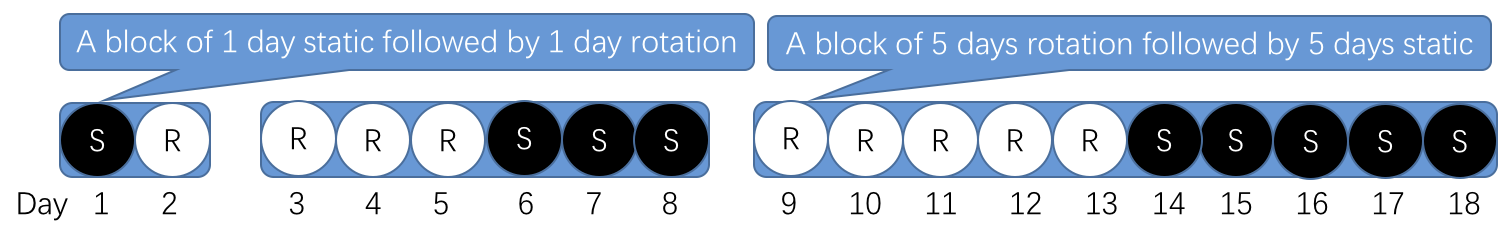
\includegraphics[width=1.0\textwidth]{figures/experiment1_design_figure_v2.png}
	\caption{Example order in which a user might see conditions. Each circle represents a day -- on black days the user is in the ``static'' condition, white is the ``rotation'' condition. The order of blocks is randomized; here, this participant is seeing blocks in order 1, then 3, then 5, then 7 (omitted in the figure).}
\label{fig:experiment1_design_figure}
\end{figure}

The experimental unit was a participant assigned to a condition for a block of days. Block lengths were randomized between 1 day, 3 days, 5 days, and 7 days, in order to give us insight into the effects of rotation strategy over different time horizons. When participants were randomized to a block, for example a five-day block, they experienced HabitLab in one condition for five days, then in the other condition for five days, for a total of ten days (Figure~\ref{fig:experiment1_design_figure}). Condition order was randomized within each block. At the conclusion of a block, the user was then moved into another block length and the trial repeated. The sequence of block lengths was randomized for each participant. If they kept the system installed, participants would experience all blocks after 32 days.

\subsection{Conditions}
We developed a within-subjects repeated measures design, where users alternated between blocks of time during which they were shown either a static intervention or rotated interventions. A within-subjects design such as this allows us to better control for the large variability across users in how much time they spend on a site.

The static condition captures a typical behavior change design with one strategy. At install time, for each site, the participant is randomly assigned a single intervention among the ones that are enabled for the site. Whenever they visit that site on a day in the static condition, the participant will always see that intervention, \rev{i.e. the static intervention is the same across all blocks.}

The rotation condition captures a strategy of keeping the interventions changing so that users do not begin ignoring them. Each time a participant in the rotation condition visits a target site (e.g., Facebook), HabitLab picks a random intervention from the enabled set to display.

So, in a five day block, a user might spend five days in the static condition seeing the same intervention each time, then five days in the rotation condition seeing randomly selected interventions each time. They are then moved into another block and the method repeats.

\subsection{Measures}

We measured the \textit{effectiveness} of the system as the number of seconds spent on the target site each day. Time, of course, does not perfectly correspond to attention or engagement behavior, as users can get distracted and not actually attend to a web page. However, prior work has generally found it to be an effective estimate (e.g.,~\cite{whittaker2016don}). %We refine our time tracker to measure time the same way that the Chrome browser does: active time is counted as the tab focused, window focused, and mouse or keyboard movement within the past minute. 
To determine whether the user is actively using a target site, we use Chrome's internal definition of active --- the browser window and tab is focused, the computer screen is on, and there has been mouse or keyboard activity on the tab within the past minute. 
%We aggregate our measurements at two levels: sessions and days. Time on site per session is measured as the total time the user was actively using a site in a browser tab, from when they visited the site until they closed the tab.
%If the user switches tabs to a different site, the time spent on the other site is not counted towards the current session time. 
Time on site per day is measured as the aggregated time across sessions from midnight to midnight in the participant's local timezone.
There was %one session data point per user per session per web site, and 
one data point per user per day per targeted web site.
Because time data is not normally distributed, we adopt a common practice of log-transforming the time data prior to analysis.


%We measured \textit{attrition} as the number of days the participant kept the extension enabled. We also noted if the extension was still enabled at the conclusion of our study. The browser does not reliably send a notification to our server if a user disables or uninstalls the extension, so we coded instances of attrition when the server stopped receiving data from the user for over two days, with no later resumption.

We measured \textit{attrition} as the number of days the participant kept the extension enabled. We also noted if the extension was still enabled at the conclusion of our study. The browser does not send a notification to our server if a user disables the extension, so we coded instances of attrition when the server stopped receiving data from the user for over two days, with no later resumption.

As with many online field experiments, effective data cleaning is essential to accurate analysis. We excluded users who had HabitLab installed on multiple devices, to focus on site usage on a single device. %For measurements of time on site per day, w
We discarded days on which the target site was never visited, as in neither condition would the intervention have been shown. %For measurements of time on site per day, w
We also discarded the first day because participants installed the extension midway through the day, resulting in an underestimate at the day level; we likewise discarded any days on which the user uninstalled or disabled the extension, as this would again cause the measured time to be an underestimate of the actual time spent on site that day.

\subsection{Method of Analysis}

For analyzing effectiveness at both the day and session level, we used a linear mixed model (LMM). We used an LMM because we have multiple samples from each user, but the number of samples from each user and in each condition is variable (because attrition may occur before they completed all conditions, or they may not visit a site on a particular day), which violates the assumptions of the repeated-measures ANOVA. 

%Upon installation, users chose which sites they want HabitLab to track. Because users spend differing amounts of time on different domains, and there was a long tail of domains which were set as goal sites by only a few users, we restricted analysis to the top 5 domains that our participants marked as wanting to spend less time on: Facebook, Youtube, Reddit, Twitter, and VK (a Russian social network).

To test whether interventions decrease in effectiveness over time (H\ref*{hyp:decreaseovertime}), we focused on just data points from the static condition. The model included a term for the number of days that particular intervention had previously been seen,\footnote{\rev{Repeating the analysis using the number of times the intervention had been seen yields the same conclusions.}} a random effect for the participant, and a random effect for domain. To test linear mixed models for significance, we used a likelihood ratio test to compare a reduced model without the number of days predictor to the full model. A significant test indicates that the number of days has statistically significant explanatory power, analogous to a significant beta coefficient in a traditional regression.

To test whether static or rotated interventions increase effectiveness (H\ref*{hyp:rotation}), we used data from both the static and rotation conditions. This second LMM, predicting log time spent on the site each day, included a random effect for participant, a random effect for domain, a fixed effect for block length, and a fixed effect for condition. A likelihood ratio test compared to a reduced model without the condition variable. 

To analyze whether static or rotated interventions increase attrition (H\ref*{hyp:attrition}), we %used a pair of analyses. First, a generalized linear mixed model (GLMM) predicted whether attrition would occur after each session. Because attrition is a binary variable in this context, a GLMM with binomial (logistic) link function is more appropriate than an LMM. The model included the same predictors as above, and is also tested against a reduced model using a likelihood ratio test. 
%To analyze attrition effects over longer (block-length) periods, we 
used a Cox proportional hazards regression. Cox proportional hazards models predict the relative ``hazard'' (i.e. risk) of attrition given each predictor. This is used in the health sciences for estimating expected lifetimes when we may have differing durations of observations for each participant, and may have observed deaths (which correspond to attrition) for some participants but not others. Each data point consists of a point of observation, and whether the participant had experienced attrition at that point or was still active. To avoid crossing conditions in this analysis, we focus the Cox analysis on just each user's first assigned block and condition, for example a seven-day rotation block or three-day static block. Each observation consists of the length of block, and whether the user had experienced attrition by the end of the first condition for their first block. The Cox model used a single predictor: condition. The output of a Cox proportional hazards model is similar to a regression, with a significance value and estimate attached to the predictor.

% \section{Study 1 Methodology}

% We used a within-subjects repeated measures design, where users alternated between blocks of time during which they were shown either the same intervention for N days (where N is selected randomly from either 1,3,5, or 7), or random interventions each visit for N days, followed by the opposite condition (random counterbalanced). We chose a within-subjects design because there is extreme variability in how much time users spend on each site, making this unsuitable for a between-subjects design. Users were assigned. Due to natural user attrition over time and the fact that 

% 196 users installed HabitLab over the course of our experiment, but we discarded users who were not new users of HabitLab (some users were reinstalls or new devices for existing users), and we discarded users who stopped using the system within the first day (the majority of attritions occur within the first 5 minutes, due to users installing extensions simply to explore and compare them). Our analysis will focus only on users who used our Facebook interventions, which leaves us with 55 users.

% Users were divided into . Exact demographics are unknown but Google Analytics estimates that X\% of visitors to the HabitLab website are (fill in). Users are globally distributed from (fill in).
